\subsubsection{Listar}

  \paragraph{}Para mostrar esta lista, es necesario establecer el asesor para
  el que mostrar sus preguntas disponibles. Para ello, habrá que elegir
  el asesor en la lista desplegable que se muestra en la figura
  \ref{capturaPantallaSelectAsesor}.

  \paragraph{}También habrá que seleccionar el curso académico para el que
  listar las preguntas del asesor seleccionado. La figura
  \ref{capturaPantallaSelectAsesorCursoAcademico} muestra una captura de
  pantalla de la lista desplegable para seleccionarlo.

  \paragraph{}Por último, es necesario establecer la plantilla de asesor para la
  que mostrar las preguntas disponibles. Para ello, habrá que elegir la
  plantilla en la lista desplegable que se muestra en la
  figura \ref{capturaPantallaSelectPlantillaAsesor}.

  \begin{figure}[!ht]
    \begin{center}
      \fbox{
      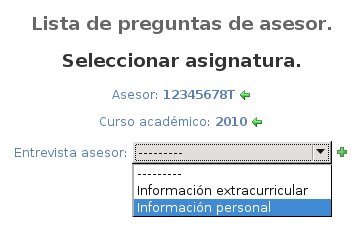
\includegraphics[scale=0.55]{4.Funcionamiento_Aplicacion/4.3.Gestion/4.3.1.Administrador_Principal/4.3.1.21.PreguntaAsesor/select_plantilla.png}
      }
      \caption{Captura de pantalla de la lista desplegable para seleccionar plantilla de asesor para el usuario \textit{Administrador principal}.}
      \label{capturaPantallaSelectPlantillaAsesor}
    \end{center}
  \end{figure}

  \paragraph{}Nótese que si no existieran elementos disponibles en el sistema,
  la lista desplegable aparecería vacía. Por tanto, se proporciona al usuario
  un icono, representado por una cruz verde, para añadir nuevos elementos al
  sistema. Este icono es el mostrado en la figura \ref{capturaBotonAdd}. Al
  pulsar dicho botón, aparecerá la ventana de creación de un nuevo elemento.

  \paragraph{}Una vez seleccionada la plantilla de asesor de entre las
  disponibles, se muestra la lista completa de preguntas que aparecen en el
  sistema. La figura \ref{capturaPantallaListaPreguntasAsesorAdminPrincipal}
  muestra una captura de pantalla de la lista de preguntas de asesor.

  \begin{figure}[!ht]
    \begin{center}
      \fbox{
      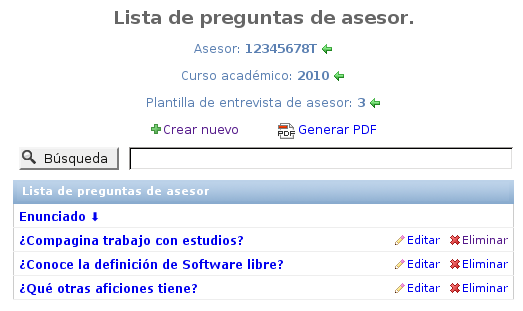
\includegraphics[scale=0.55]{4.Funcionamiento_Aplicacion/4.3.Gestion/4.3.1.Administrador_Principal/4.3.1.21.PreguntaAsesor/lista_preguntas_asesor.png}
      }
      \caption{Captura de pantalla de la lista de preguntas de asesor para el usuario \textit{Administrador principal}.}
      \label{capturaPantallaListaPreguntasAsesorAdminPrincipal}
    \end{center}
  \end{figure}
